        	\begin{question}{1201}{Vecteurs}{1}{1220}
				Dans un repère à deux dimensions, quelles sont les coordonnées du vecteur allant du point $(0;0)$ au point $(1;2)$?
            \end{question}
            \begin{reponses}
            	\item[false] $(-1;-2)$
            	\item[false] $(2;1)$
                \item[false] $(-2;-1)$
                \item[true] $(1;2)$
            \end{reponses}
			%%%%%%%%%%%%%%%%%%%%%%%%%%%%%%%%%%%%%
            \begin{question}{1201}{Vecteurs}{2}{1220}
                Quelles sont les coordonnées du vecteur $\vec{AB}$?
                \begin{center}
                	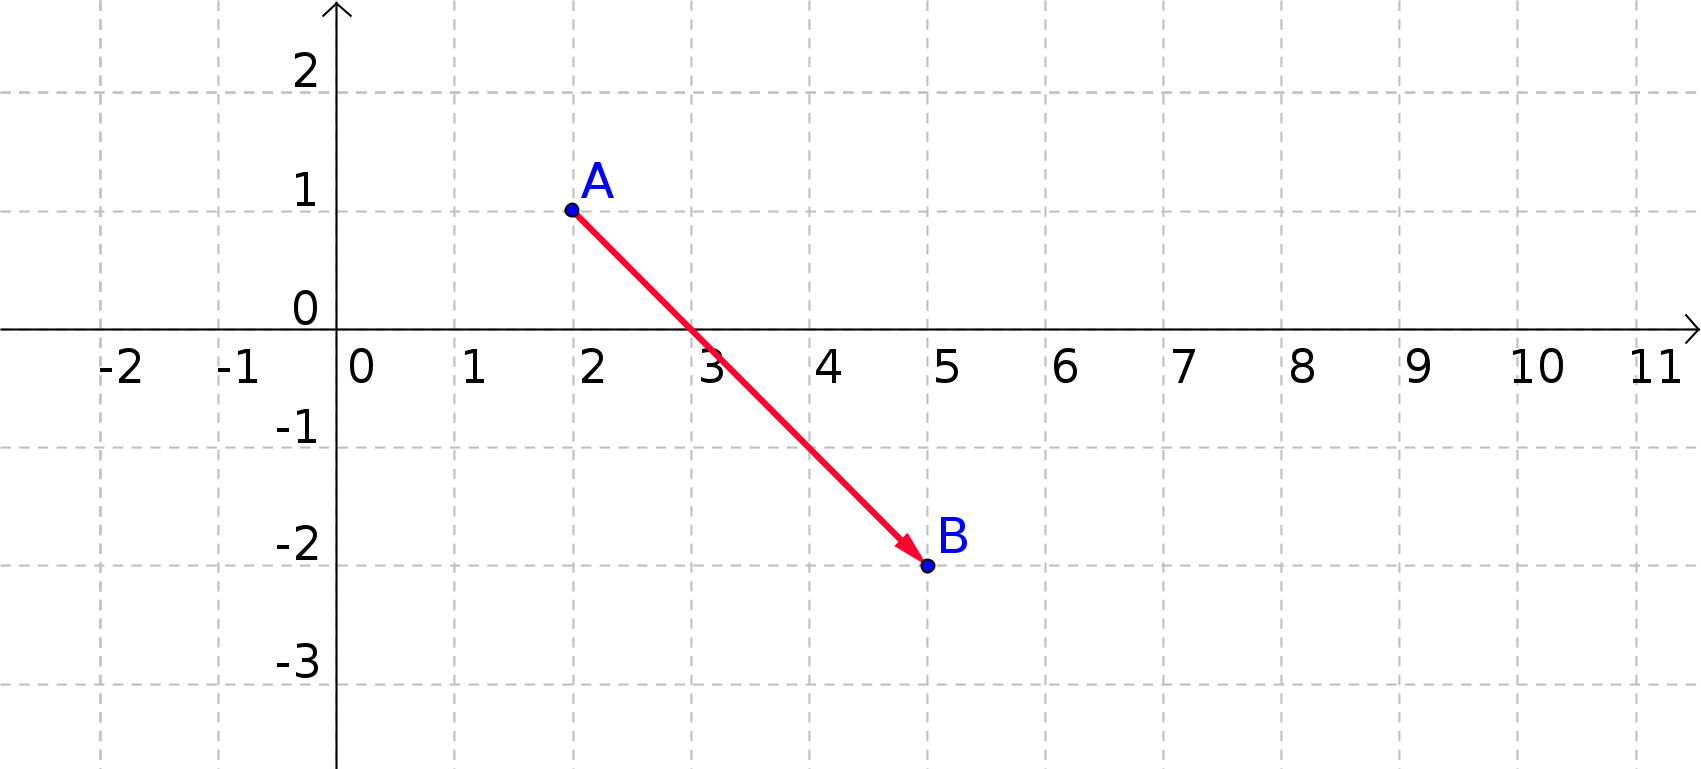
\includegraphics[width=0.5\textwidth]{Philippe/Figures_Philippe/vecteurs_4_3.png}
                \end{center}
            \end{question}
            \begin{reponses}
                \item[false] $(5;-2)$
                \item[false] $(3;3)$
                \item[false] $(-3;3)$
                \item[true] $(3;-3)$ 
            \end{reponses}
            %%%%%%%%%%%%%%%%%%%%%%%%%%%%%%%%%%%%%
            \begin{question}{1201}{Vecteurs}{2}{1220}
                Dans l'espace à trois dimensions, quelles sont les coordonnées du vecteur allant du point $(12;-2;6)$ au point $(-1;0;3)$?
            \end{question}
            \begin{reponses}
                \item[true] $(-13;2;-3)$
                \item[false] $(13;-2;3)$
                \item[false] $(11;2;9)$
                \item[false] $(11;2;3)$
            \end{reponses}
            %%%%%%%%%%%%%%%%%%%%%%%%%%%%%%%%%%%%%
            \begin{question}{1201}{Vecteurs}{2}{1220}
                On donne la position du centre de la Terre comme étant en $(200;542;865)$ et la position d'un satellite en $(-412;-102;623)$. Quelles sont les coordonnées du vecteur reliant le centre de la Terre au satellite?
            \end{question}
            \begin{reponses}
                \item[false] $(612;644;242)$
                \item[false] $(-212;440;242)$
                \item[false] $(212;-440;-242)$
                \item[true] $(-612;-644;-242)$
            \end{reponses}
            %%%%%%%%%%%%%%%%%%%%%%%%%%%%%%%%%%%%%
            \begin{question}{/}{Vecteurs}{2}{1217,31,1213}
                Que valent les coordonnées $x$ et $y$ du vecteur $\vec{OM}$ ci-dessous? \\ 
            \begin{tikzpicture}[scale=3, axis/.style={->,blue,thick}, vector/.style={-stealth,red,very thick}, vector guide/.style={dashed,red,thick}]
                \coordinate[label=below  left:O] (O) at (0cm,0cm);
                \coordinate[label=below  left:] (x) at (1cm,0cm);
                \draw[axis] (0,0) -- (1,0) node[anchor=north east]{$x$};
                \draw[axis] (0,0) -- (0,1) node[anchor=north west]{$y$};
                \draw[-Stealth] (O) to ["$OM=3$",sloped] ++ (150.0:3) coordinate[label=above right:M] (M);
                \draw[densely dotted] (O) to ["$x$"] ++ (0:-2.59) coordinate (Mx);
                \draw[densely dotted] (Mx) to ["$y$"] ++ (90:1.5);
                \pic ["$\theta=5\pi/6$", draw=red,->, angle radius = 12mm, angle eccentricity=1.3] {angle = x--O--M};
            \end{tikzpicture}
            \end{question}
            \begin{reponses}
                \item[false] $x$ = $3\sqrt{3}$ et $y$ = $-3$
                \item[false] $x$ = $-3$ et $y$ = $0$
                \item[false] $x$ = $3\sqrt{2}/2$ et $y$ = $-3\sqrt{2}/2$
                \item[true] $x$ = $-3\sqrt{3}/2$ et $y$ = $3/2$
            \end{reponses}
